
\section{Teknologibeskrivelse}
Aktivitetsarmbånd bliver i stigende grad mere udbredt. Ifølge IDC er der sket en stigning i salget af aktivitetsarmbånd fra 11,8 millioner enheder i første kvartal af 2015 til 19,7 millioner i første kvartal af 2016 \citep{IDC2016}.

Det har ikke været muligt at finde statistisk data vedrørende udbredelsen af fitbit flex armbåndet. Det ses dog at Fitbit udgør stor andel af markedet for aktivitetsarmbånd, og at der fra første kvartal i 2015 til første kvartal i 2016 er sket en stigning i salget på 1 million enheder \citep{IDC2016}.  

\begin{figure}[H]
	\centering
	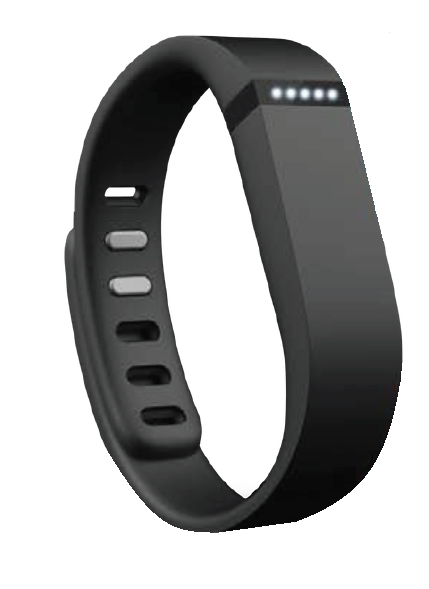
\includegraphics[width=0.35\textwidth]{figures/fitbitflex}
	\caption{Fitbit flex armbånd \citep{fitbitflex}.}
	\label{fig:fitbitflexarmbånd}
\end{figure}


Overordnet består et Fitbit Flex aktivitetsarmbånd af en flex tracker, oplader kabel, trådløs synkroniserings dongle og armbånd til flex tracker \citep{fitbitflex}. Disse kan ligeledes ses af \autoref{fig:fitbitflexindhold}. 

\begin{figure}[H]
	\centering
	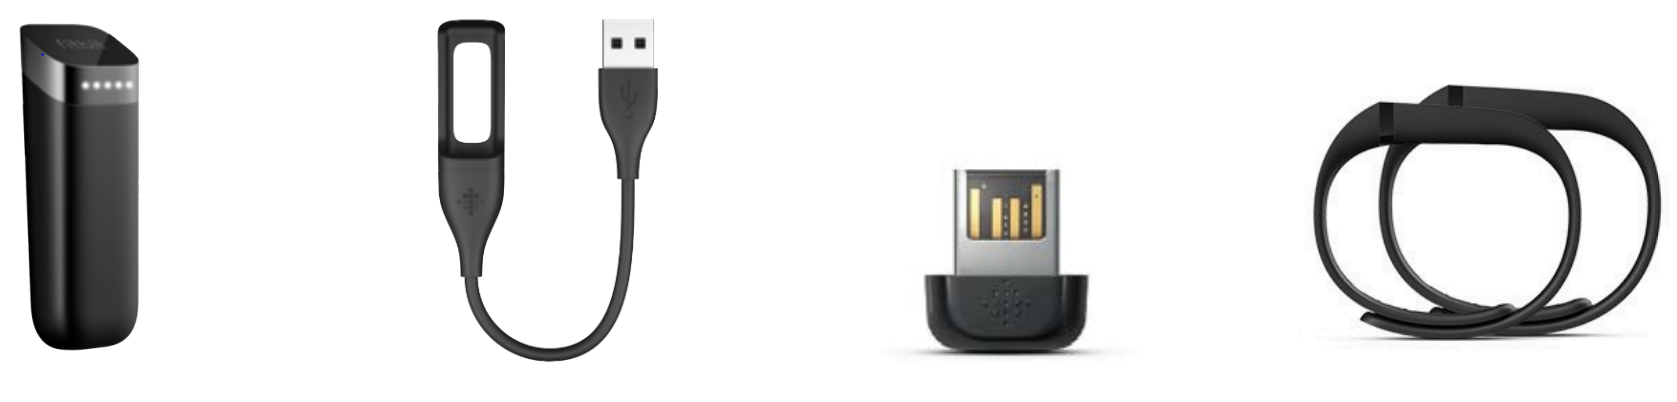
\includegraphics[width=0.6\textwidth]{figures/fitbitflexindhold}
	\caption{Fra venstre mod højre ses flex tracker, oplader kabel, trådløs synkroniserings dongle, armbånd \citep{fitbitflex}.}
	\label{fig:fitbitflexindhold}
\end{figure}

Fitbit Flex er i stand til at måle antal skridt, forbrændte kalorier, afstand dækket, minutter brugeren er aktiv og længden samt kvalitet af søvn. 
For at brugeren kan se den registrerede aktivitet, som er blevet opsamlet af armbåndet, skal dette synkroniseres med en kompatibel enhed, da armbåndet kun besidder et display bestående af fem LED'er. %(HVAD BETYDER DET SÅ?? HVIS DER ER 5 STYREDE LED'ER HVAD VISES SÅ??)  
Synkronisering foregår trådløst, ved brug af bluetooth low energy og kan foregå mellem forskellige enheder som for eksempel smartphone og computer. 
Synkronisering mellem flex tracker og computer kræver dog anvendelse af den trådløs synkroniserings dongle, der ses af \autoref{fig:fitbitflexindhold}.
Forudsætninger for, at data kan synkroniseres er, at en kompatibel enhed har den korrekte applikation installeret, hvor synkroniseringen ellers sker automatisk idet applikationen åbnes.  
Yderligere skal der oprettes en brugerkonto på www.fitbit.com, hvor brugeren oplyser personlig info: køn, alder, højde og vægt. Dette er nødvendigt i forhold til optimering af dataopsamling og estimering af forbrændte kalorier.  
Gennem applikationen visualiseres den registrerede aktivitet, hvor brugeren har mulighed for at se data fra starttidspunktet for anvendelsen af armbåndet. Data kan også observeres via  Fitbits hjemmeside, hvor det er muligt at logge ind via brugerkontoen. 
Til den daglige aktivitet har brugeren mulighed for at sætte bestemte mål, hvortil det angives, hvor langt brugeren er fra at nå det givne fysiske mål, ved hjælp af de fem LED'er på armbåndet, i løbet af dagen. Denne funktion aktiveres når brugeren trykker 2 gange på armbåndet. 
Når et af brugerens mål gennemføres, visualiseres dette ved at de 5 LED'er blinker og at armbåndet vibrerer. 
Fitbit Flex armbåndet er ikke i stand til at visualisere batteriniveauet for armbåndet, dette kan dog ses ved brug af applikationen. 
Hukommelsen i flex trackeren tillader detaljeret data at blive lagret i perioder op til 7 dage og består af minut til minut målinger.  
Yderligere lagres summeringer af daglig aktivitet i op til 30 dage. 
%(VIL DET SIGE AT HVIS MAN IKKE SYNKRONISERER, SÅ LAGRES DATA PÅ ENHEDEN, OG EFTER 7 DAGE SLETTES DEN FØRSTE AF DE 7 DAGE (GEMMES MÅSKE SOM EN SUMMERING AF DAGEN FOR DE 30 DAGE) ELLER HVORDAN FUNGERER DET? : jaa hvordan man.)) 
Ved jævnlig synkronisering er det muligt for brugeren at bevare detaljeret data, da informationen tilknyttes brugerkontoen. 
Fitbit anbefaler én daglig synkronisering, dog er det ikke en nødvendighed \citep{fitbitflex}. 

Armbåndet er vandafvisende. \textbf{KOMMER UD AF INGENTING}


% Hvordan udregnes de reelle trackingsværdier, kalorier, afstand mm. 

\subsection{Hardware}
Fitbit flex trackeren har forskellige hardware elementer, hvorfra trackeren signalere, og detektere fysisk aktivitet. Hardwaren i trackeren udgøres af et display, sensor, motorer og batteri.
 
\textbf{Display:} 
Flex trackeren er udstyret med fem LED'er, der ved forskellige operationstilstande signalerer til brugeren. 
LED'erne fungerer for eksempel, som indikator for progressionen i forhold til det brugerdefinerede fysiske mål for dagen. Hertil vil hver LED repræsentere en procentvis progressionen i intervaller af $20 \%$. Eksempelvis hvis brugeren har opfyldt $73 \%$ af det fysisk mål, vil de første tre LED'er lyse og den fjerde vil blinke. Dette indikerer, at brugeren har nået $60 \%$ af målet, og at brugeren nu befinder sig mellem $60 \%$ og $80 \%$. 
Det samme gør sig gældende når flex trackeren sættes til opladning. Her indikerer LED'erne, hvor langt armbåndet er fra fuld opladning, som signaleres ved at alle fem LED'er lyser. 
I tilfælde af synkroniseringsfejl vil dette også fremgå af LED'erne. Her vil armbåndet lyse med et mønster, skiftevis mellem at have ingen eller alle LED'er tændt. 
Ved manuel aktivering og de-aktivering af sleep mode, vil LED'erne indikere dette gennem forskellige indikationsmønstre.

\textbf{Sensor:} 
Flex trackeren registrer den fysiske aktivitet ved anvendelse af et MEMS 3-akses accelerometer, hvilket er den eneste sensor, som sidder i armbåndet. Ud fra algoritmer analyseres bevægelsesmønstre, hvorved der kan oplyses hvor mange skridt der er foretaget under løb eller gang, den tilbagelagte afstand, med mere. 

\textbf{Motorer:}
Flex trackeren er yderligere udstyret med en vibrationsmotor, der aktiveres under forskellige funktioner når armbåndet anvendes. Disse fungerer i sammenspil med displayet, som et kommunikationsredskab for brugeren. Vibration aktiveres ved anvendelse af alarm funktion og ved aktivering eller de-aktivering af sleep mode, samt når det daglige fysiske mål nåes. 
 
\textbf{Batteri:} 
Fitbit Flex indeholder et genopladeligt batteri, der lades ved brug af det medfølgende kabel. Dette ses af \autoref{fig:fitbitflexindhold}. Kablet tilsluttes en computer og opladningen begynder, hvis computeren er tændt. 
Levetiden på batteriet er op til 5 dage, dog kan mindre forventes ved omstændigt brug.


\subsection{Software}
\textbf{MANGLER INDLEDNING}

Alt efter brugerens engagement, kan der også udfyldes informationer omkring indtaget kost ved brug af applikationen. Brugeren kan ud fra dette få et estimat af hvor mange kalorier der indtages, hvortil dette kan sammenlignes med antal kalorier forbrændt. Anvendelsen af denne kost-log er dog ikke en nødvendighed for anvendelsen af armbåndet eller applikationen, dog kunne dette give en praktiserende læge indblik i om patienten overholder anbefalingerne for hypertensive patienter, både i forhold til kostvaner, samt fysisk aktivitet.  

\begin{figure}[H]
	\centering
	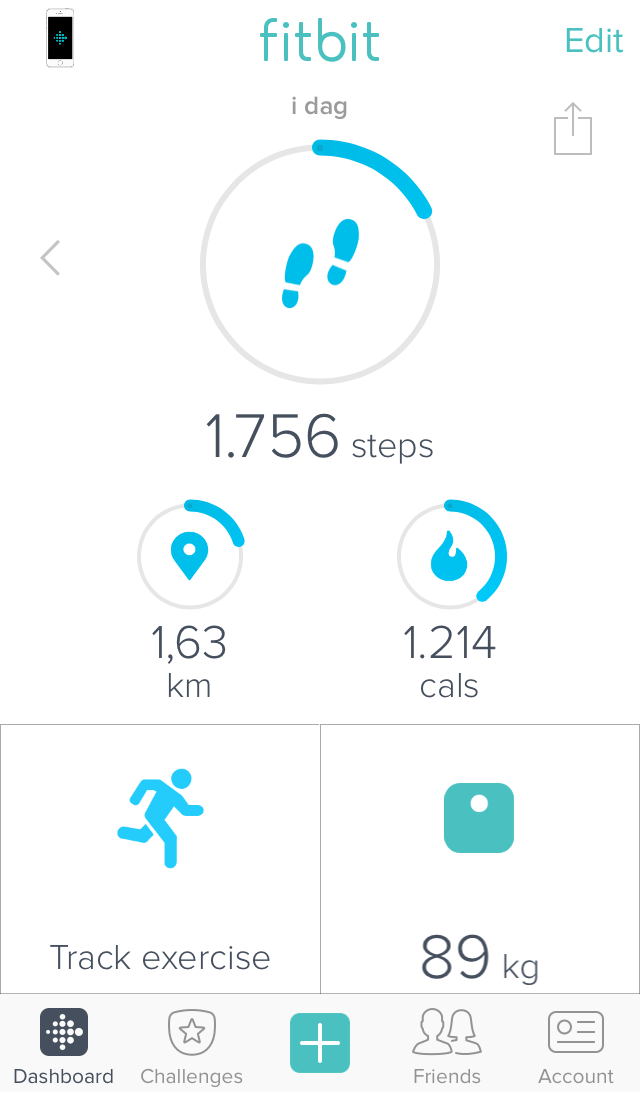
\includegraphics[width=0.45\textwidth]{figures/burgerfladeoversigt}
	\caption{Oversigt af fysisk aktivitet, der vises idet applikationen åbnes. Her vises antal skridt taget, afstand rejst, kalorier forbrændt med mere.}
	\label{fig:brugerfladeoversigt}
\end{figure}

Af \autoref{fig:brugerfladeoversigt} ses oversigt over den registrerede aktivitet som er målt gennem armbåndet. Her ses skridt taget, afstand rejst og kalorier forbrændt. Af oversigten ses også hvor langt brugeren er fra at opfylde de forskellige aktivitetsmål, og er repræsenteret af den blå cirkel omkring de forskellige angivelser. 
Af bunden ses fire forskellige oversigter, hvor der fra venstre mod højre ses dashboard, udfordringer, tilføjelser, fællesskab og brugerkonto. \textbf{Dashboardet} er den overordnede oversigt, som oplyser det førnævnte (ydet aktivitet). 
\textbf{Udfordringer} viser en oversigt over tilvalgte aktivitetsudfordringer, hvor brugeren har mulighed for at opstille udfordringer med venner samt andre brugere af applikationen. 
\textbf{Tilføjelser} tillader ændringer af kost-loggen, eller opstart af ny aktivitetsmåling. 
\textbf{Fællesskab} giver brugeren et overblik og venner der er tilføjet til applikationen. 
\textbf{Brugerkonto} viser overblik over hvilken bruger der er logget ind, og hvilken enhed er der synkroniseret med applikationen. Yderligere kan der fortages ændringer af profil og mål for daglig fysisk aktivitet. 

En detaljeret oversigt over ydet aktivitet kan ses under den overordnet oversigt, ved at tykke på de givne målinger. Ved at trykke på skridt ses eksemplet der fremgår af \autoref{fig:brugerfladesteps}.  

\begin{figure}[H]
	\centering
	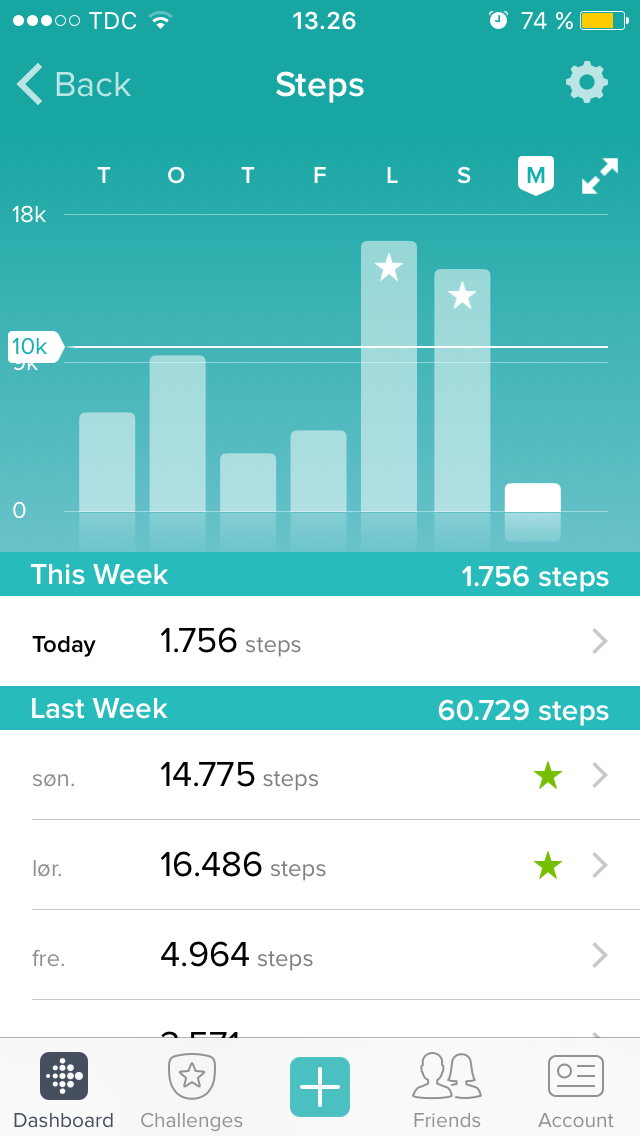
\includegraphics[width=0.45\textwidth]{figures/brugerfladesteps}
	\caption{Til venstre ses den grafiske oversigt over antal skridt taget, og højre figur viser skridt taget i en tabel.}
	\label{fig:brugerfladesteps}
\end{figure}

Af \autoref{fig:brugerfladesteps} ses der foroven en graf over skridt taget inden for den sidste uge. Af grafen ses en hvid tværgående linje, der repræsenterer målet for skridt. Hertil ses at dage hvor målet er blevet opfyldt markeres med en stjerne.  

Under grafen ses en oversigt over antal skridt taget for de forhenværende dage, rækkende tilbage til den første anvendelsesdato. Heraf ses ligeledes at dagene hvor målet nås, er indikeret med en stjerne. Ved at trykke på den give dag eller en af de forhenværende dage, kan der ses en mere detaljeret oversigt skridt taget i løbet af dagen. Dette ses af \autoref{fig:specifiksteps}, hvor der er muligt at se hvilke tider at dagen brugeren er mest aktiv.  

\begin{figure}[H]
	\centering
	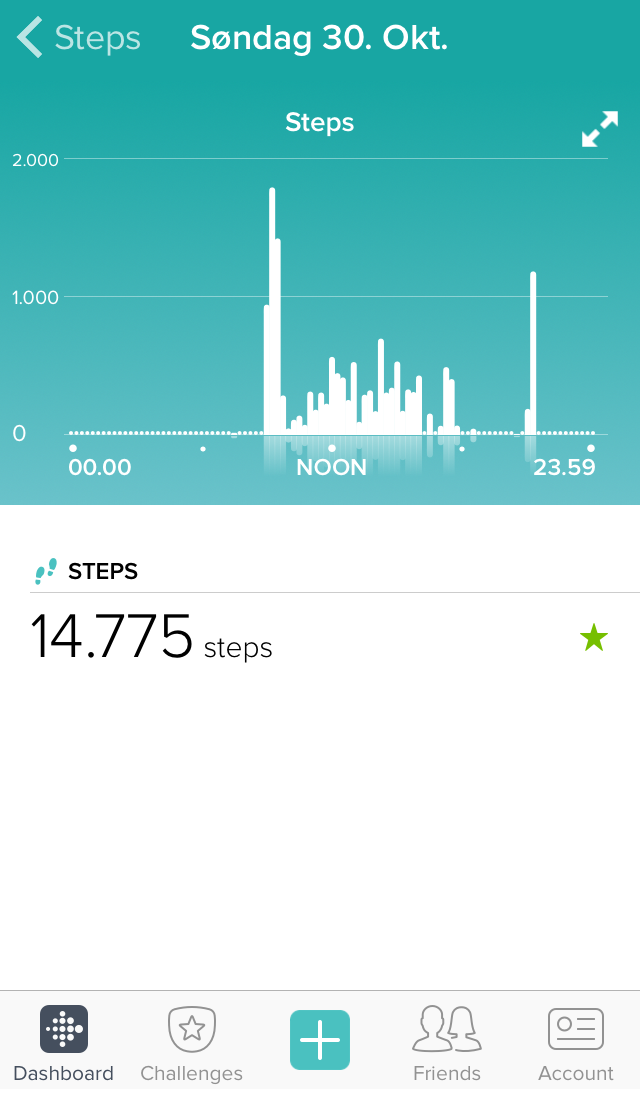
\includegraphics[width=0.45\textwidth]{figures/specifiksteps}
	\caption{Til venstre ses den grafiske oversigt over antal skridt taget, og højre figur viser skridt taget i en tabel.}
	\label{fig:specifiksteps}
\end{figure}


\subsection{Brugertilpasning}
Der er forskellige muligheder for at tilpasse armbåndet optimalt til den givne bruger. Heriblandt er der mulighed og at udskifte armbåndet til andre længder, og at tilpasse skridtlængden til den enkelte bruger. 

\subsubsection{Forskellige størrelser armbånd}
For brugeren er der mulighed for at vælge mellem to forskellige længder af armbånd. Dette tillader muligheden for bedre tilpasning omkring håndleddet. Armbåndene kan ligeledes fås i forskellige farver. % Swag 

\subsubsection{Kalibrering}
Som standard vurderer applikationen brugerens skridtlængde, ud fra de angivne oplysninger ved oprettelsen af brugerkontoen. Brugeren har dog mulighed for at kalibrerer denne værdi, i tilfælde af at brugeren opdager uoverensstemmelse mellem registrerede værdier og reelle værdier. Brugeren kan under indstillinger i applikationen ændre den pre-defineret skridtlængde, til en mere passende. Fitbit oplyser på deres support-hjemmeside guidelines for hvordan brugeren selv udregner værdier til en mere passende skridtlængde.   

\begin{comment}
%	\end{itemize}
%	\item Hvor udbredt er teknologien? (Studier med noget statistik hertil.)
Producenten Fitbit 			
			
 Statistik op aktivitetsarmbånd på verdensplan 
%	\item Aktivitetsarmbånd
%	\begin{itemize}
%		\item Hvilke sensor bliver brugt til at opsamle data
%		\item Et billede hertil!
%	\end{itemize}
%	\item Hvordan monteres/påføres teknologien 
%	\item Hvordan kalibreres teknologien til den enkelte person?
%	\begin{itemize}
%		\item Skal der udføres nogle test for at vide f.eks. hvilepulsen hos patienten? i så fald hvordan gøres dette?
%	\end{itemize}
%	\item Levetid for teknologien (Evt. Batterilevetid/Totale levetid)
%	\item Hvordan lagres og videregives informationen til en læge?
%\end{itemize}
\end{comment}
